%*******10********20********30********40********50********60********70********80
\subsection{Uni-axial compression result for $10 \times 10 \times 10$ mm DEF Expanded Models}

Simulation of uni-axial compression test on a single aggregate case in size $10 \times 10 \times 10$ mm is presented also for DEF damaged concrete model (Figure \ref{cdefsma}). Same as in ASR case, in each step of loading, the top boundary of the concrete model moves downwards 0.002 mm.

The model is expanded by DEF following the process in chapter 2 and 3. 0.0003 initial strain is given to all paste interfaces uniformly in this simulation. Totally 20 steps of expansion are done.

%TODO: Single Aggregate 3D, 2D

\begin{figure}[h!]
\centering
%*******
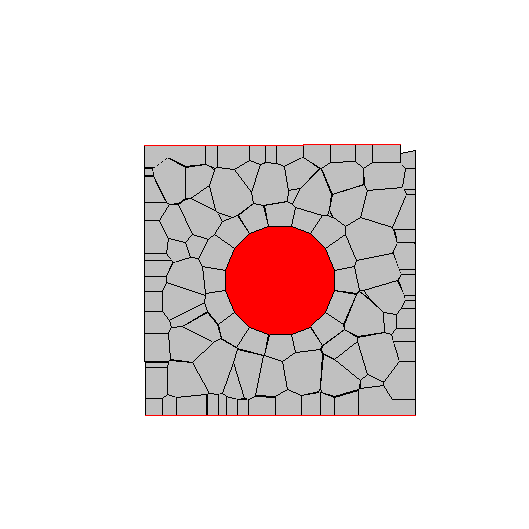
\includegraphics[width=0.4\linewidth]{Files/Small_DEF/CR/DEP5-STEP(001).png}
\caption{Single Aggregate Case in Size $10 \times 10 \times 10$ mm}
\label{cdefsma}
\end{figure}

\begin{figure}[ht!]
\centering

    %*******
    \begin{subfigure}{.33\textwidth}
      \centering
      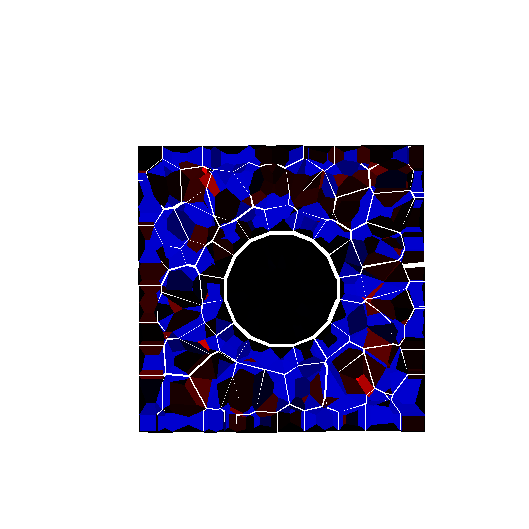
\includegraphics[width=1.0\linewidth]{Files/Small_DEF/IS2/DEP5-STEP(020).png}
      \caption{Before Loading}
    \end{subfigure}%
    \begin{subfigure}{.33\textwidth}
      \centering
      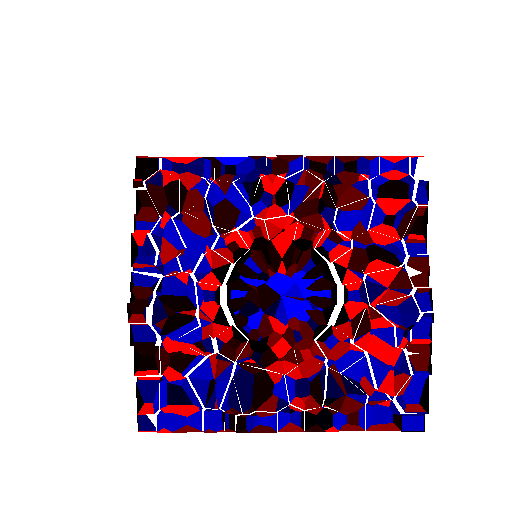
\includegraphics[width=1.0\linewidth]{Files/Small_DEF/IS2/DEP5-STEP(040).png}
      \caption{Loading Step 20}
      \end{subfigure}%
      %*******
      \begin{subfigure}{.33\textwidth}
        \centering
        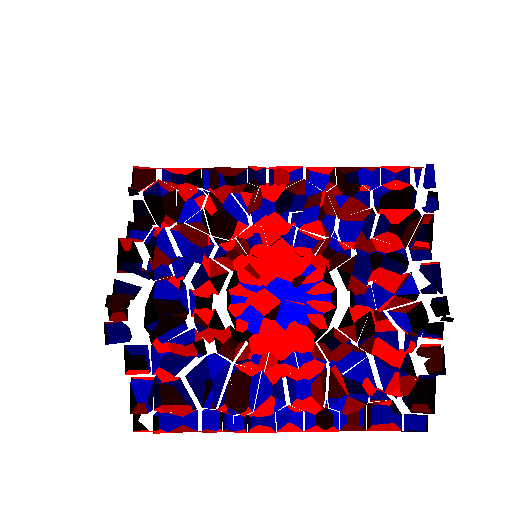
\includegraphics[width=1.0\linewidth]{Files/Small_DEF/IS2/DEP5-STEP(060).png}
        \caption{Loading Step 40}
      \end{subfigure}
      %*******

    %*******
    \begin{subfigure}{.33\textwidth}
      \centering
      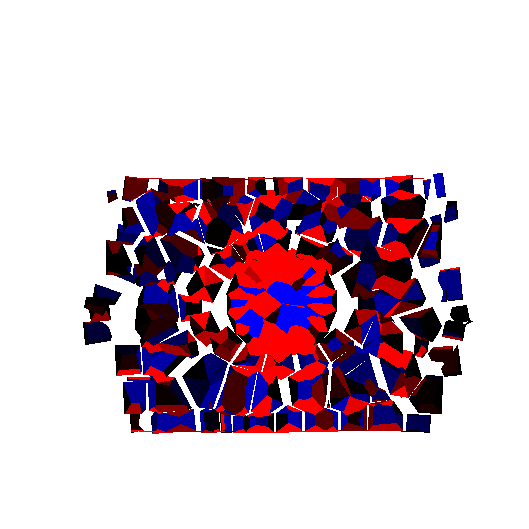
\includegraphics[width=1.0\linewidth]{Files/Small_DEF/IS2/DEP5-STEP(080).png}
      \caption{Loading Step 60}
    \end{subfigure}%
    \begin{subfigure}{.33\textwidth}
      \centering
      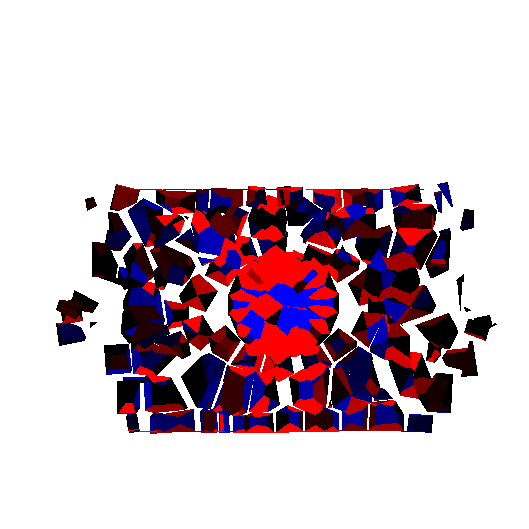
\includegraphics[width=1.0\linewidth]{Files/Small_DEF/IS2/DEP5-STEP(100).png}
      \caption{Loading Step 80}
      \end{subfigure}%
      %*******
      \begin{subfigure}{.33\textwidth}
        \centering
        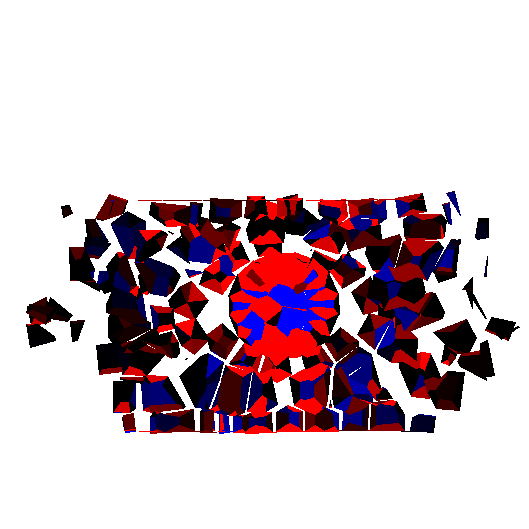
\includegraphics[width=1.0\linewidth]{Files/Small_DEF/IS2/DEP5-STEP(120).png}
        \caption{Loading Step 100}
      \end{subfigure}
      %*******
  \begin{subfigure}{0.8\textwidth}
  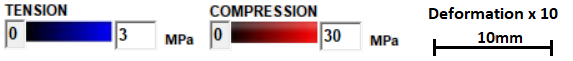
\includegraphics[width=0.8\linewidth]{Files/exp_3D/tagCS30s.png}
\end{subfigure}%

  \caption{DEF Loading for $10 \times 10 \times 10$ mm model, Fixed Boundary Condition}
  \label{fig:DEF_Loading_s_fix}
\end{figure}

For Loading with fixed boundary condition, Figure \ref{fig:DEF_Loading_s_fix} here shows the initial stress condition during loading in loading step 0, 20, 30, 60 and 80.

With increasing the step of loading, in each step the top surface moves downwards for 0.002 mm. Compressive strength generate together with the deformation, especially concentrated horizontally in the middle of the model.

As the top and bottom boundary are horizontally, elements in the middle of model start to move away from the center of model firstly, followed by the failure of whole model.

If we compare its behavior with free boundary condition loading, shown in Figure \ref{fig:DEF_Loading_s_free}, it can be seen that the way crack generate and deformation generate is totally different in these two cases.

In Free boundary loading, the cracks are more easier to open without the restrain from top and bottom boundary. The deformation in horizontal direction is more uniformed. Inner Stress distributed more uniformly in the free boundary loading case.

\begin{figure}[ht!]
\centering

    %*******
    \begin{subfigure}{.33\textwidth}
      \centering
      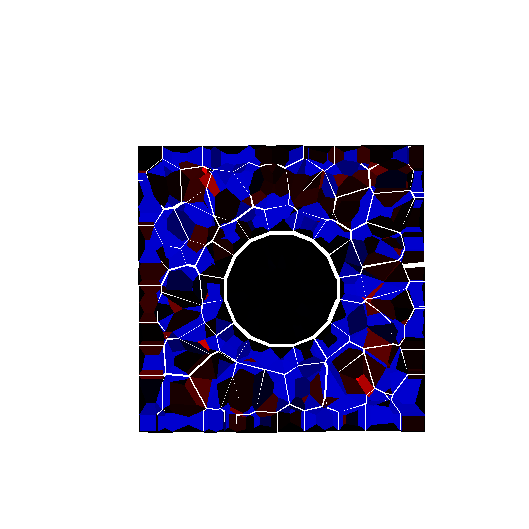
\includegraphics[width=1.0\linewidth]{Files/Small_DEF/IS2/DEP5-STEP(020).png}
      \caption{Before Loading}
    \end{subfigure}%
    \begin{subfigure}{.33\textwidth}
      \centering
      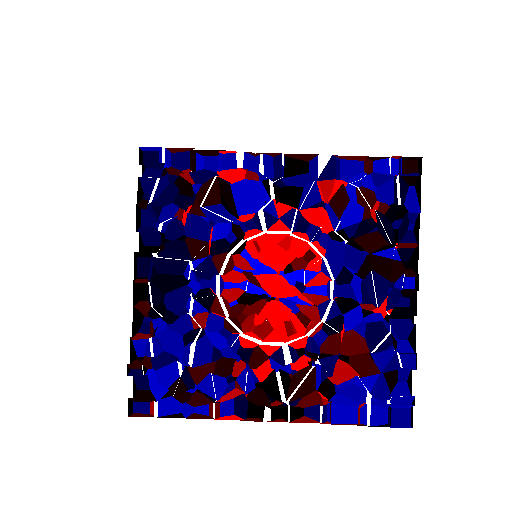
\includegraphics[width=1.0\linewidth]{Files/Small_DEF/Free_IS2/DEP5-STEP(040).png}
      \caption{Loading Step 20}
      \end{subfigure}%
      %*******
      \begin{subfigure}{.33\textwidth}
        \centering
        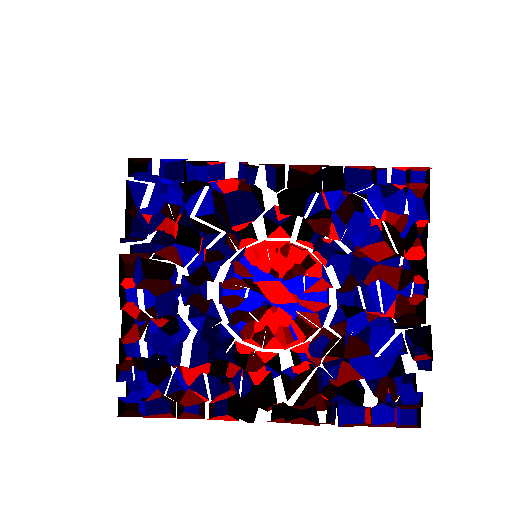
\includegraphics[width=1.0\linewidth]{Files/Small_DEF/Free_IS2/DEP5-STEP(060).png}
        \caption{Loading Step 40}
      \end{subfigure}
      %*******

    %*******
    \begin{subfigure}{.33\textwidth}
      \centering
      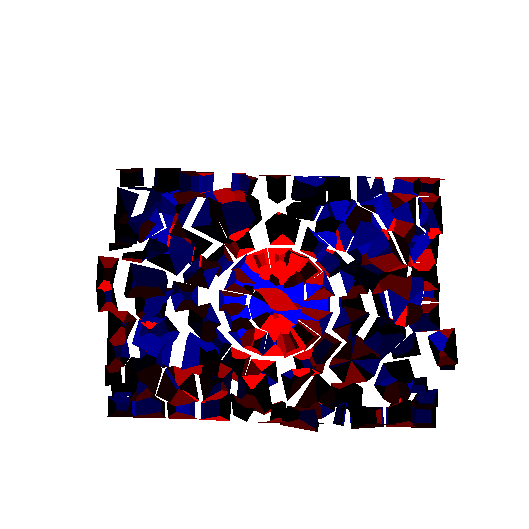
\includegraphics[width=1.0\linewidth]{Files/Small_DEF/Free_IS2/DEP5-STEP(080).png}
      \caption{Loading Step 60}
    \end{subfigure}%
    \begin{subfigure}{.33\textwidth}
      \centering
      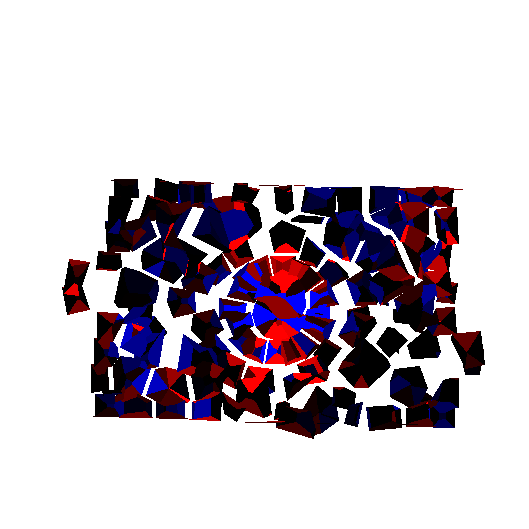
\includegraphics[width=1.0\linewidth]{Files/Small_DEF/Free_IS2/DEP5-STEP(100).png}
      \caption{Loading Step 80}
      \end{subfigure}%
      %*******
      \begin{subfigure}{.33\textwidth}
        \centering
        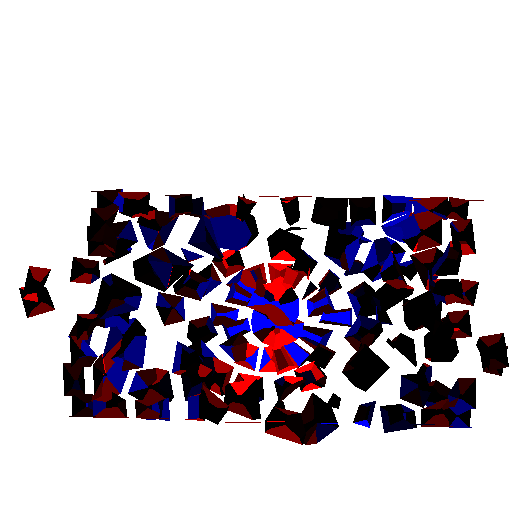
\includegraphics[width=1.0\linewidth]{Files/Small_DEF/Free_IS2/DEP5-STEP(120).png}
        \caption{Loading Step 100}
      \end{subfigure}
      %*******
  \begin{subfigure}{0.8\textwidth}
  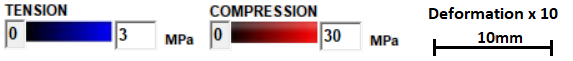
\includegraphics[width=0.8\linewidth]{Files/exp_3D/tagCS30s.png}
\end{subfigure}%

  \caption{DEF Loading for $10 \times 10 \times 10$ mm model, Free Boundary Condition}
  \label{fig:DEF_Loading_s_free}
\end{figure}

Later, uni-axial compression test on full size model($100 \times 100 \times 100$ mm) damaged by DEF expansion will also be carried out.
